% Pour toute question sur l'utilisation de cette classe, écrivez à jerome.soucy(at)ulaval.ca
% Nécessite la classe Evaluation.sty dans le même dossier ou dans le PATH de votre système
% Nécessite le fichier logo_ul.pdf dans le même dossier un dans le PATH de votre système
\def\Ponderation{35}
\def\SigleNumero{STT-2100}
\def\NomCours{Régression}
\def\DateEvaluation{12 décembre 2024}
\def\DateRemise{}
\def\HeureRemise{}
\def\HeureEvaluation{10h30 à 12h20}
\def\Session{Été 2021}
\def\NomEvaluation{Examen 2}

% Ne rien mettre entre les accolades si l'enseignant (ou l'enseignante) est aussi le coordonnateur (ou la coordonnatrice)
\def\Coordonnatrice{}
\def\Coordonnateur{}

% Ne rien mettre entre les accolades s'il y a plus d'une section
\def\Enseignant{}
\def\Enseignante{Audrey-Anne Vallée}

% Ne rien mettre entre les accolades s'il s'agit d'un cours à section unique
% Mettre le nom de chacun des enseignants et enseignantes entre les accolades
% Une case à cocher sera générée pour chacune des sections
\def\SectionA{}
\def\SectionB{}
\def\SectionC{}
\def\SectionD{}


\def\Directives{
\begin{enumerate}
\item Matériel autorisé:
\begin{itemize}
\item Calculatrice scientifique {\bf autorisée par la FSG};
\item Le feuillet de formules est fourni avec l'examen. Celui-ci inclut les tables de lois. Veuillez ne rien écrire sur le feuillet de formules.
\end{itemize}
\item Assurez-vous que cette évaluation comporte \numquestions ~exercices répartis sur \numpages{}~pages, pour un total de \numpoints{}~points.\
\item \textbf{Veuillez ne pas dégrafer votre examen.}
\item Ajoutez vos initiales dans le bas de chaque page de l'examen.
\item Veuillez déposer votre carte d'identité \textbf{admise} avec photo sur votre bureau.\
\item {\bf Vous devez justifier chaque réponse, soit par une démarche, soit par une (des) phrase(s). Justifiez toutes les étapes de vos démarches.}
\item  Le verso des feuilles peut être utilisé comme brouillon, \textbf{mais ne sera pas corrigé}. Attention à ne rien dégrafer.
\end{enumerate}
}

\documentclass[Examen]{Evaluation}
\usepackage{multicol,graphicx}
\begin{document}

\begin{questions}  

\question 
Pour chaque énoncé qui suit, indiquez s'il est vrai ou faux.
\textbf{Justifiez} brièvement votre réponse. Il peut s'agir d'une justification mathématique ou d'une phrase. \\
\textit{Aucun point ne sera accordé pour une réponse sans justification ou une mauvaise justification.}

\vspace{0.3cm}
\begin{parts}
\part[4]  Dans un modèle de régression linéaire multiple, la valeur-p du test F ajusté associé à une
variable explicative est toujours plus grande que celle du test t partiel de cette même variable.

     \begin{oneparcheckboxes}
		\choice VRAI
		\correctchoice FAUX
\end{oneparcheckboxes}

\begin{solution}
    Elles sont égales, les tests sont équivalents.
\end{solution}



\part[4] Yves veut modéliser le temps requis pour cuire un gâteau au chocolat en fonction de différentes variables explicatives. Il cuisine plusieurs gâteaux en faisant varier les valeurs des variables explicatives. Pour un des gâteaux, il a noté un temps de cuisson de 530 minutes plutôt que 53 minutes. Cette observation, lorsqu'incluse dans l'estimation du modèle de régression linéaire multiple, sera forcément influente.

     \begin{oneparcheckboxes}
		\choice VRAI
		\correctchoice FAUX
\end{oneparcheckboxes}

\begin{solution}
    L'erreur est en Y, pas en X. Il se peut que le levier soit petit et qu'elle ne soit pas influente.
\end{solution}



\part[4] Le coefficient de détermination ($R^2$) est un outil approprié pour faire la sélection de variables à inclure dans le modèle.

     \begin{oneparcheckboxes}
		\choice VRAI
		\correctchoice FAUX
\end{oneparcheckboxes}

\begin{solution}
Il augmente lorsque $p$ augmente, donc non.
\end{solution}



\part[4] La valeur minimale du facteur d'inflation de la variance est 0. 

     \begin{oneparcheckboxes}
		\choice VRAI
		\correctchoice FAUX
\end{oneparcheckboxes}

\begin{solution}
$\frac{1}{1-R_j^2}$

$=1 si R_j^2 = 0$ et augmente si $R_j^2$ augmente.

Donc 1.
\end{solution}

\end{parts}


\newpage

\question
Pour chaque énoncé qui suit, justifiez brièvement votre réponse. Il peut s'agir d'une justification mathématique ou d'une phrase. \\

\begin{parts}
\part[4] Pourquoi doit-on faire attention de ne pas inclure des variables inutiles dans un modèle de régression linéaire multiple?

\begin{solution}
    Ça fait augmenter la variance des estimateurs des coefficients de régression et des prévisions.
\end{solution}

\part[4] Pourquoi la matrice des corrélations entre les variables indépendantes n’est pas suffisante pour diagnostiquer la multicolinéarité?

\begin{solution}
Elle n'identifie que les problèmes impliquant 2 variables explicatives, pas ceux impliquant plus de 2 variables explicatives.    
\end{solution}


\part[4] Soit le modèle de régression linéaire multiple pour lequel tous les postulats sont respectés. Calculez la covariance entre $\boldsymbol{Y}$ et $\boldsymbol{\varepsilon}$, c'est-à-dire $\mathrm{Cov}(\boldsymbol{y}, \boldsymbol{\varepsilon})$.

\begin{solution}
    $\mathrm{Cov}(y, \varepsilon) 
    = \mathrm{Cov}(X\beta+\varepsilon, \varepsilon)
    = \mathrm{Cov}(\varepsilon, \varepsilon)
    = = \mathrm{Var}(\varepsilon)
    = \sigma^2 \bf{1}$
\end{solution}


\part[4] Que puis-je faire si j’ai un problème avec le postulat de linéarité et que je n’arrive pas à le corriger avec des transformations des variables? Donnez deux suggestions.

\begin{solution}
    Régression polynomiale, régression splines, arbres de régression
\end{solution}


\end{parts}


\newpage

\question\label{matrices}
On examine la réponse d'une variable $Y$ en fonction de deux variables explicatives $x_1$ et $x_2$, à partir d'un échantillon. Soit $\boldsymbol{X}=(\boldsymbol{1}, \boldsymbol{x}_1, \boldsymbol{x}_2)$ une matrice $n\times 3$, où $\boldsymbol{1}$ est le vecteur de 1 associé à l'ordonnée à l'origine. 
Voici la matrice $(\boldsymbol{X}^T\boldsymbol{X})^{-1}$ et la matrice des corrélations entre toutes les variables.
Notons $\beta_1$ et $\beta_2$ les coefficients associés aux variables ${x}_1$ et ${x}_2$.
On s'intéresse à estimer le modèle
$$ Y_i = \beta_0 + \beta_1 x_{i1} + \beta_2 x_{i2} + \varepsilon_i, $$
dans lequel les postulats de la régression linéaire sont respectés.

\bigskip

$
(\boldsymbol{X}^T\boldsymbol{X})^{-1}=\left[
\begin{array}{ccc}
  0.71 &-0.34 & 0.03\\
 -0.34 & 0.35& -0.12\\
  0.03 &-0.12 & 0.10\\
\end{array}\right]\qquad
Corr=\begin{array}{c}
X_1 \\
X_2  \\
Y \\
\end{array}\left[
\begin{array}{rrr}
  1.00 & 0.65& -0.10\\
  0.65 & 1.00 &-0.72\\
 -0.10 &-0.72 & 1.00\\
\end{array}\right]
$

\medskip

\begin{parts}
    \part[3]  Donnez la valeur du facteur d'inflation de la variance associé à $x_2$. Justifiez votre réponse.
 
    \begin{solution}
         $corr = 0,65 $
         
     $R^2 = 0,65^2 = 0,4225$
     
     $VIF_2 = 1/(1-0,4225) = 1,7316$
    \end{solution}
    
    \part[3] En supposant que $\widehat{\sigma}^2 = 1$, que vaut $\widehat{\mathrm{Var}}(\widehat{\beta}_1)$, l'estimateur de la variance de $\widehat{\beta}_1$? Justifiez votre réponse.

\begin{solution}
        $1 \times 0,35$
    \end{solution}
    
    \part[3] En supposant que $\widehat{\sigma}^2 = 1$, que vaut $\widehat{\mathrm{Cov}}(\widehat{\beta}_1, \widehat{\beta}_2)$, l'estimateur de la covariance entre $\widehat{\beta}_1$ et~$\widehat{\beta}_2$? Justifiez votre réponse.


    \begin{solution}
        $1 \times -0,12$
    \end{solution}
\end{parts}

\newpage
\question\label{interactionEThypotheses}
On s'intéresse au succès des personnes étudiantes à leur première année universitaire en fonction de leur présence en classe et de leur cote Z. Pour 150 étudiants ayant terminé leur première année, on a :
\begin{itemize}
    \item $Y_i$ = la moyenne globale de l’étudiant $i$ après sa première année universitaire;
    \item $p_i$ = la présence en classe de l'étudiant $i$ (toujours présent, quelques fois présent, souvent absent);
    \item $z_i$ = la cote $Z$ de l'étudiant $i$.
\end{itemize}
Le modèle de régression  est 
\begin{equation}\label{eq:modeleInteraction}
    Y_i=\beta_0 + \beta_Z z_i + \beta_{T} t_{i} + \beta_Q q_i + \beta_{ZT}t_i z_i+ \beta_{ZQ}q_i z_i + \varepsilon_i,
\end{equation}
où 
\begin{align*}
    t_i =\left\{
			\begin{array}{ll}
			1  & \mbox{ si $i$ est toujours présent}, \\
			0 & \mbox{ sinon, }
   \end{array}
			\right. & & q_i =\left\{
			\begin{array}{ll}
			1  & \mbox{ si $i$ est quelques fois présent}, \\
			0 & \mbox{ sinon. }
   \end{array}
			\right. 
\end{align*}

\vspace{0.25cm}
\begin{parts}
    \renewcommand*\half{,5}
\part[7\half]
Voici des énoncés basés sur le modèle (\ref{eq:modeleInteraction}):
\medskip

\begin{enumerate}
    \item La moyenne globale ne dépend pas de la présence en classe.
    % $ \beta_T = \beta_Q = \beta_{ZT} = \beta_{ZQ} = 0 $
    \item La moyenne globale ne dépend pas de la cote Z.
    % $ \beta_Z = \beta_{ZT} = \beta_{ZQ} = 0  $ 
    \item L'effet d'une hausse de 0,5 unité de la cote Z sur la moyenne globale est le même peu importe la présence en classe. 
    % $ \beta_{ZT} = \beta_{ZQ} = 0 $
    \item Il n'y a aucun lien linéaire entre la moyenne globale et les variables explicatives (ni leur intéraction); 
    % $ \beta_Z = \beta_T = \beta_Q = \beta_{ZT} = \beta_{ZQ} = 0  $
    \item L'espérance de la moyenne globale est de $0$, lorsque $z_i=0$ et $t_i=1$.
    % $ \beta_0 = \beta_T = 0 $
\end{enumerate}

\medskip\medskip

 Pour chacun des énoncés ci-haut, cochez l'hypothèse qui correspond.


\begin{solution}
\begin{tabular}{|c||ccccc|}
\hline
& \multicolumn{5}{c|}{Énoncés}\\ \hline
Hypothèses & \multicolumn{1}{l||}{~~~1~~~} & \multicolumn{1}{l||}{~~~2~~~} & \multicolumn{1}{l||}{~~~3~~~} & \multicolumn{1}{l||}{~~~4~~~} & \multicolumn{1}{l||}{~~~5~~~} \\ \hline
%%%
$ \beta_Z = \beta_T = \beta_Q = \beta_{ZT} = \beta_{ZQ} = 0  $ & \multicolumn{1}{l||}{}  & \multicolumn{1}{l||}{}  & \multicolumn{1}{l||}{}  & \multicolumn{1}{l||}{X}  & \multicolumn{1}{l||}{}     \\ \hline
$ \beta_0 = \beta_Z = \beta_T = \beta_Q = \beta_{ZT} = \beta_{ZQ} = 0  $ & \multicolumn{1}{l||}{}  & \multicolumn{1}{l||}{}  & \multicolumn{1}{l||}{}  & \multicolumn{1}{l||}{}  & \multicolumn{1}{l||}{}     \\ \hline
$ \beta_Z + 0,5 = 0 $ & \multicolumn{1}{l||}{}  & \multicolumn{1}{l||}{}  & \multicolumn{1}{l||}{}  & \multicolumn{1}{l||}{}  & \multicolumn{1}{l||}{}     \\ \hline
$ \beta_Z = 0 $ & \multicolumn{1}{l||}{}  & \multicolumn{1}{l||}{}  & \multicolumn{1}{l||}{}  & \multicolumn{1}{l||}{}  & \multicolumn{1}{l||}{}     \\ \hline
$ \beta_T = 0 $ & \multicolumn{1}{l||}{}  & \multicolumn{1}{l||}{}  & \multicolumn{1}{l||}{}  & \multicolumn{1}{l||}{}  & \multicolumn{1}{l||}{}     \\ \hline
$ \beta_Z = \beta_{ZT} = \beta_{ZQ} = 0  $ & \multicolumn{1}{l||}{}  & \multicolumn{1}{l||}{X}  & \multicolumn{1}{l||}{}  & \multicolumn{1}{l||}{}  & \multicolumn{1}{l||}{}     \\ \hline
$ \beta_{ZT} = \beta_{ZQ} = 0 $ & \multicolumn{1}{l||}{}  & \multicolumn{1}{l||}{}  & \multicolumn{1}{l||}{X}  & \multicolumn{1}{l||}{}  & \multicolumn{1}{l||}{}     \\ \hline
$ \beta_T = \beta_Q = 0 $ & \multicolumn{1}{l||}{}  & \multicolumn{1}{l||}{}  & \multicolumn{1}{l||}{}  & \multicolumn{1}{l||}{}  & \multicolumn{1}{l||}{}     \\ \hline
$ \beta_T = \beta_Q = \beta_{ZT} = \beta_{ZQ} = 0 $ & \multicolumn{1}{l||}{X}  & \multicolumn{1}{l||}{}  & \multicolumn{1}{l||}{}  & \multicolumn{1}{l||}{}  & \multicolumn{1}{l||}{}   \\ \hline
$ \beta_0 = 0 $ & \multicolumn{1}{l||}{}  & \multicolumn{1}{l||}{}  & \multicolumn{1}{l||}{}  & \multicolumn{1}{l||}{}  & \multicolumn{1}{l||}{}     \\ \hline
$ \beta_0 = \beta_T = 0 $ & \multicolumn{1}{l||}{}  & \multicolumn{1}{l||}{}  & \multicolumn{1}{l||}{}  & \multicolumn{1}{l||}{}  & \multicolumn{1}{l||}{X}     \\ \hline
\end{tabular}
\end{solution}

\newpage

\part[2\half] À partir du modèle (\ref{eq:modeleInteraction}), l'espérance de la moyenne globale d'une personne augmente de combien d'unités si sa cote Z vaut 5 unités de plus? Justifiez votre réponse.
% 5\beta_z + 5\beta_{ZT}t_i + 5\beta_{ZQ}q_i

\begin{solution}
    \begin{align*}
    \mathrm{E}(Y_i) &= \beta_0 + \beta_Z z_i + \beta_{T} t_{i} + \beta_Q q_i + \beta_{ZT}t_i z_i+ \beta_{ZQ}q_i z_i \cr 
    \mathrm{E}(Y_i|z_i+5) &= \beta_0 + \beta_Z (z_i+5) + \beta_{T} t_{i} + \beta_Q q_i + \beta_{ZT}t_i (z_i+5)+ \beta_{ZQ}q_i (z_i+5) \cr 
    diff &=  5\beta_Z  + 5\beta_{ZT}t_i + 5\beta_{ZQ}q_i 
\end{align*}
\end{solution}

\part[5] À partir du modèle (\ref{eq:modeleInteraction}), tracez un graphique de l'espérance de $Y$.
Notez que le graphique n'a pas besoin d'être parfait, ni à l'échelle.
Par contre, on doit y retrouver les éléments importants, les coefficients du modèle et le nom des axes. Supposez que tous les coefficients sont non nuls et de valeurs différentes.

\begin{solution}
Y ~ Z

3 droites

3 ordonnées

3 pentes    
\end{solution}


\end{parts}


\newpage

\question\label{demonstration}
Soit le mod\`ele de r\'egression lin\'eaire 
$$\boldsymbol{Y}=\boldsymbol{X}\boldsymbol{\beta}+\boldsymbol{\varepsilon},$$
o\`u $\mathrm{E}(\boldsymbol{\varepsilon}) = {\bf 0}$ et $\mathrm{Var}(\boldsymbol{\varepsilon})=\sigma^2 \boldsymbol{A} $, $\sigma>0$ et  $\boldsymbol{A}$ est une matrice sym\'etrique de dimension $n\times n$. Posons $\widetilde{\boldsymbol{\beta}}=(\boldsymbol{X}^\top\boldsymbol{X})^{-1}\boldsymbol{X}^\top\boldsymbol{Y}$.

\begin{parts}
	\part[5] Montrez que $\widetilde{\boldsymbol{\beta}}$ est un estimateur non biais\'e de $\boldsymbol{\beta}$. Justifiez toutes les étapes de votre démarche.

    \begin{solution}
        \begin{align*}
            \mathrm{E}(\widetilde{\boldsymbol{\beta}})
            &= \mathrm{E} ((\boldsymbol{X}^\top\boldsymbol{X})^{-1}\boldsymbol{X}^\top\boldsymbol{Y}) \cr
            &= (\boldsymbol{X}^\top\boldsymbol{X})^{-1}\boldsymbol{X}^\top \mathrm{E} (\boldsymbol{Y}) \cr
            &= (\boldsymbol{X}^\top\boldsymbol{X})^{-1}\boldsymbol{X}^\top \mathrm{E} (\boldsymbol{X}\boldsymbol{\beta}+\boldsymbol{\varepsilon}) \cr
            &= (\boldsymbol{X}^\top\boldsymbol{X})^{-1}\boldsymbol{X}^\top (\boldsymbol{X}\boldsymbol{\beta}+\mathrm{E} (\boldsymbol{\varepsilon}) )\cr
            &= (\boldsymbol{X}^\top\boldsymbol{X})^{-1}\boldsymbol{X}^\top (\boldsymbol{X}\boldsymbol{\beta}+\bf{0})\cr
             &= (\boldsymbol{X}^\top\boldsymbol{X})^{-1}\boldsymbol{X}^\top \boldsymbol{X}\boldsymbol{\beta}\cr
             &= \boldsymbol{\beta}\cr
        \end{align*}
    \end{solution}
    
	\part[7] Calculez la variance de $\widetilde{\boldsymbol{\beta}}$ et donnez son expression. Justifiez toutes les étapes de votre démarche.

    \begin{solution}
        \begin{align*}
            \mathrm{Var}(\widetilde{\boldsymbol{\beta}})
            &= \mathrm{Var} ((\boldsymbol{X}^\top\boldsymbol{X})^{-1}\boldsymbol{X}^\top\boldsymbol{Y}) \cr
            &= (\boldsymbol{X}^\top\boldsymbol{X})^{-1}\boldsymbol{X}^\top \mathrm{Var} (\boldsymbol{Y}) ((\boldsymbol{X}^\top\boldsymbol{X})^{-1}\boldsymbol{X}^\top )^\top \cr
            &= (\boldsymbol{X}^\top\boldsymbol{X})^{-1}\boldsymbol{X}^\top \mathrm{Var} (\boldsymbol{X}\boldsymbol{\beta}+\boldsymbol{\varepsilon}) \boldsymbol{X}(\boldsymbol{X}^\top\boldsymbol{X})^{-1} \cr
            &= (\boldsymbol{X}^\top\boldsymbol{X})^{-1}\boldsymbol{X}^\top \mathrm{Var} (\boldsymbol{\varepsilon}) \boldsymbol{X}(\boldsymbol{X}^\top\boldsymbol{X})^{-1} \cr
             &= (\boldsymbol{X}^\top\boldsymbol{X})^{-1}\boldsymbol{X}^\top \sigma^2 \boldsymbol{A}  \boldsymbol{X}(\boldsymbol{X}^\top\boldsymbol{X})^{-1} \cr
              &=  \sigma^2 (\boldsymbol{X}^\top\boldsymbol{X})^{-1}\boldsymbol{X}^\top\boldsymbol{A}  \boldsymbol{X}(\boldsymbol{X}^\top\boldsymbol{X})^{-1} \cr
        \end{align*}
    \end{solution}
    
\end{parts}

\newpage

\question[8]\label{multicolinearite}
Vous voulez ajuster une régression linéaire multiple et avez un choix de 5 prédicteurs possibles. Voici les diagnostics de multicolinérité. 

\begin{figure}[h!]
	\centering
	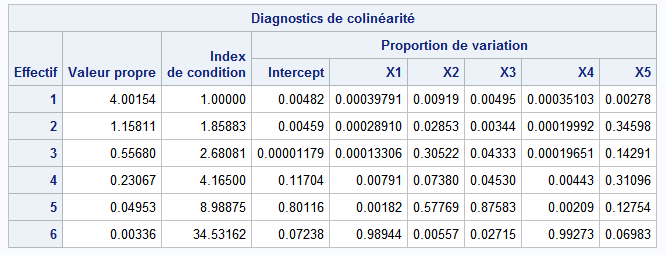
\includegraphics[scale=0.9]{multicolinearite.png}
\end{figure}

Interprétez cette sortie. Est-ce qu’un problème est détecté? Si oui, expliquez quel est le problème, quelles variables sont impliquées et ce que vous feriez par la suite. Si non, expliquez pourquoi il ne semble pas y avoir de problème. Dans vos explications, rapportez des nombres de la sortie pour justifier vos conclusions.

\begin{solution}

$\eta_6=34,53 > 30$

$\nu_{x4}= 0,98944$ et $\nu_{x1}=0,99273 > 60$

x1 et x4 multicolinéaires

enlever une des deux variables selon VIF par exemple.
\end{solution}

\newpage

\question[7]\label{selectionvariables}
Le d\'epartement
de marketing d'un magasin d'alimentation veut envoyer une publicité \`a une grande quantit\'e de m\'enages par la poste. Par contre, on ne veut envoyer
des offres qu'aux m\'enages susceptibles de g\'en\'erer de bons profits. On recueille donc des donn\'ees
sur plusieurs m\'enages par sondage t\'el\'ephonique: $Y$ est le montant d'argent d\'epens\'e
\`a l'\'epicerie \`a chaque semaine et $x_1$, $\ldots$, $x_{10}$ sont des informations
sur les m\'enages comme le niveau d'\'education des parents, le nombre d'enfants,
le type d'emploi des parents, etc. Le d\'epartement de marketing vous charge de construire
le meilleur mod\`ele de r\'egression possible afin de pr\'edire avec justesse la valeur de $Y$ en fonction
des variables exog\`enes disponibles $x_1,\ldots,x_{10}$. Vous obtenez les r\'esultats suivants:
	
	\begin{center}\begin{tabular}{|c|c|c|c|c|c|c|}\hline
			Mod\`ele & Variables incluses & $R_{a}^2$ & AIC & $C_p$ & $PRESS$ & BIC \\ \hline\hline
			1 & $x_1,x_5,x_7$ & 0.90 & 398.22 & 3.95 & 502~137 & 397.44 \\ \hline
			2 & $x_1,x_5,x_8$ & 0.85 & 397.99 & 3.95 & 752~227 & 398.54 \\\hline
			3 & $x_1,x_5$ & 0.80 & 401.65 & 2.95 & 656~123 & 397.58\\\hline
			4 & $x_1,x_5,x_7,x_8$ & 0.93 & 390.25 & 9.25 & 836~371 & 395.87 \\ \hline
	\end{tabular}\end{center}
	
	\vspace{0.1in}
	Sur la base de ce tableau, quel mod\`ele est préférable pour la mise en situation? Justifiez votre réponse, un choix de modèle non justifié ne recevra aucun points.

\begin{solution}
    modèle 1: on veut meilleures prédictions, donc $C_p-p'$ minimal et PRESS minimal.
\end{solution}
\newpage

\question[8]\label{influence}

On veut étudier le lien linéaire entre 6 variables explicatives et une variable réponse. On dispose de la sortie statistique suivante:

\begin{verbatim}
Obs   Residual   RStudent       h_ii   CovRatio     DFFITS
1      -0.184      -0.075      0.149      1.580     -0.031
2       0.114       0.047      0.175      1.632      0.022
3       2.358       1.064      0.277      1.332      0.659
4      -0.782      -2.986      0.987     10.190    -25.685
5      -3.377      -1.513      0.233      0.904     -0.833

-------------------------------------DFBETAS---------------------------
Obs  Intercept      X1        X2        X3        X4        X5        X6
1      0.011     0.002    -0.007    -0.018     0.003    -0.014    -0.002
2      0.008    -0.005    -0.001     0.011    -0.007    -0.005    -0.006
3      0.332    -0.302     0.095    -0.301    -0.102    -0.322     0.009
4      0.581    -0.351    23.385     0.413    -0.642    -0.233    -6.733
5     -0.097     0.382    -0.267    -0.338     0.317    -0.165     0.065

\end{verbatim}

Il y a eu une erreur lors de la saisie de la valeur de \texttt{X2} de l'une des 5 premières observations (on a saisi 22.3 au lieu de 223). De quelle observation s'agit-il, justifiez votre choix? Est-ce que cette observation semble potentiellement influente pour certaines inférences? Justifiez vos réponses, des réponses sans justification recevront la note 0.

\begin{solution}

    Observation 4, $h_{ii} grand$

    Influence sur variance de $\widehat{\beta}, \widehat{Y}_4, \widehat{\beta}_2, \widehat{\beta}_6$    
\end{solution}
\newpage

\question\label{application}
On s'intéresse aux infections nosocomiales (qui sont contractées dans un établissement de santé). On a collecté les variables suivantes pour un échantillon aléatoire d'hôpitaux américains:

\begin{tabular}{l|l}
	Infections & nombre moyen d'infections nosocomiales par jour \\
	StayLength & durée moyenne du séjour à l'hôpital pour tous les patients (en jours) \\
	Age & âge moyen des patients (en années) \\
	Beds & nombre de lits dans l'hôpital \\
	MedSchool & 1 si l'hôpital est affilié à une école de médecine; 0 sinon \\
	Nurses & nombre d'infirmières à temps plein
	%Region: région géographique: 1 = NorthEast, 2 = NorthCentral, 3= South, 4 = West
\end{tabular}

\vspace{0.1 in}
Vous faites l'hypothèse d'une relation linéaire entre le nombre d'infections et les autres variables. Utilisez les sorties statistiques (dans lesquelles des valeurs ont été cachées) fournies pour répondre aux questions suivantes. 

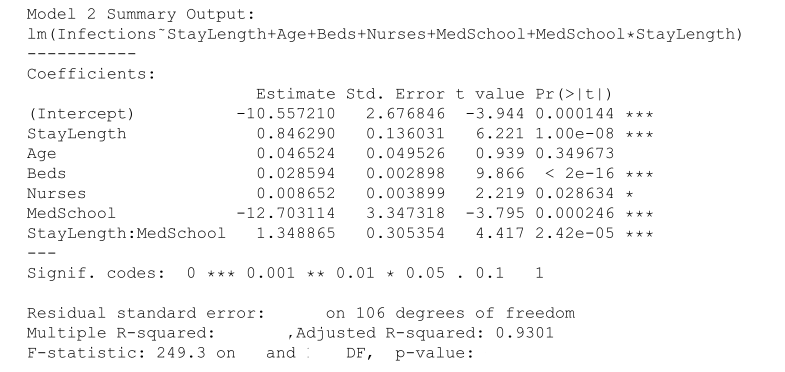
\includegraphics[scale=1]{RebeccaMod2}
 
\begin{parts}
	\part[2] Combien d'hôpitaux font partie de l'échantillon? Justifiez votre réponse.

    \begin{solution}
        $n-p' = 106$

        $n = 106 + p' = 106 + 7 = 113$
    \end{solution}

    % n-p' = 106, n-7=106, 99
	\part[3] Calculez le pourcentage de la variabilité du nombre d'infections nosocomiales qui est expliqué par le modèle.  Justifiez votre réponse.
	\begin{solution}
	    \begin{align*}
	        R^2 &= 1-\frac{SC_{res}}{SC_{tot}} \cr
            R_a^2 &= 1-\frac{SC_{res}}{SC_{tot}} \times \frac{(n-1)}{(n-p')} \cr
            0,9301 &= 1-(1-R^2)\frac{98}{106} \cr
             R^2 &= 0,9338
	    \end{align*}
	\end{solution}

    \newpage
	\part[4]  Un docteur émet l'hypothèse que l'effet de l'affiliation à une école de médecine peut dépendre de la durée moyenne du séjour des patients. Testez l'hypothèse du docteur au seuil 5\% et dites si le docteur a raison.  Justifiez votre réponse.
    \begin{solution}
        $\alpha^* = 2,45 e^{-5} < 0,05 = \alpha$

        on rejette H0.
    . Docteur a raison
    \end{solution}

	
 
	
\end{parts}


\end{questions}

\end{document}

    \part[2] En justifiant votre réponse, donnez la prévision pour un hôpital dans lequel les variables explicatives prennent les valeurs suivantes:
    
    \begin{tabular}{l|l}
    Variable & Valeur \\
    \hline
	StayLength & 3 \\
	Age & 70 \\
	Beds & 500 \\
	MedSchool & 1 \\
	Nurses & 300